\chapter{Miscellaneous} \label{ChapMisc}

%==============================================================================
\section{.bashrc Stuff}
%==============================================================================
%------------------------------------------------------------------------------
\subsection{Run \textbf{ls} after \textbf{cd}}
%------------------------------------------------------------------------------
Following `frabjous' answer to the StackOverflow question
\cite{robkohr2011make}, you can add the following to your .bashrc:
\begin{lstlisting}
function cd {
    builtin cd "$@" && ls -F
}
\end{lstlisting}
He also mentions that he adds
\begin{lstlisting}
    [ -z "$PS1" ] && return
\end{lstlisting}
before this so that ``everything after that line only applies to interactive
sessions, so this doesn't affect how \textbf{cd} behaves in scripts." How this
works is also explained by him:\\
``$[ -z "\$PS1" $] checks if the \$PS (interactive prompt variable) is `zero
length' (-z). If it is zero length, this means it has not been set, so Bash must
not be running in interactive mode. The \&\& return part exits from sourcing
.bashrc at this point, under these conditions."

%==============================================================================
\section{Ranger}
%==============================================================================
Following \cite{linuxcompendium2019ranger}:
\begin{enumerate}
    \item git clone https://github.com/hut/ranger.git
    \item cd ranger
    \item sudo make install
\end{enumerate}
To start ranger use "ranger".

%------------------------------------------------------------------------------
\subsection{Configuration}
%------------------------------------------------------------------------------
After the configuration directory has been created by the Ranger, you can now copy its configuration files by running the following commands in terminal:
\begin{itemize}
    \item "ranger --copy-config=all". Now you can run "cd ~/.config/ranger" to see the
        configuration files.
\end{itemize}

%==============================================================================
\section{Inkdrop}
%==============================================================================
\emph{Inkdrop} \cite{matsuyamainkdrop} is an absolutely incredible minimalist and
light-weight markdown-based note taking app that syncs across all devices.
It is a paid service of around \$5 a month or \$50 a year should you chose to
pay annually. It also has a convenient plugin GUI which can be accessed via the
settings menu. Since the creator is a Vim user, there is of course a Vim
plugin:
\begin{figure}[H]
    \centering
    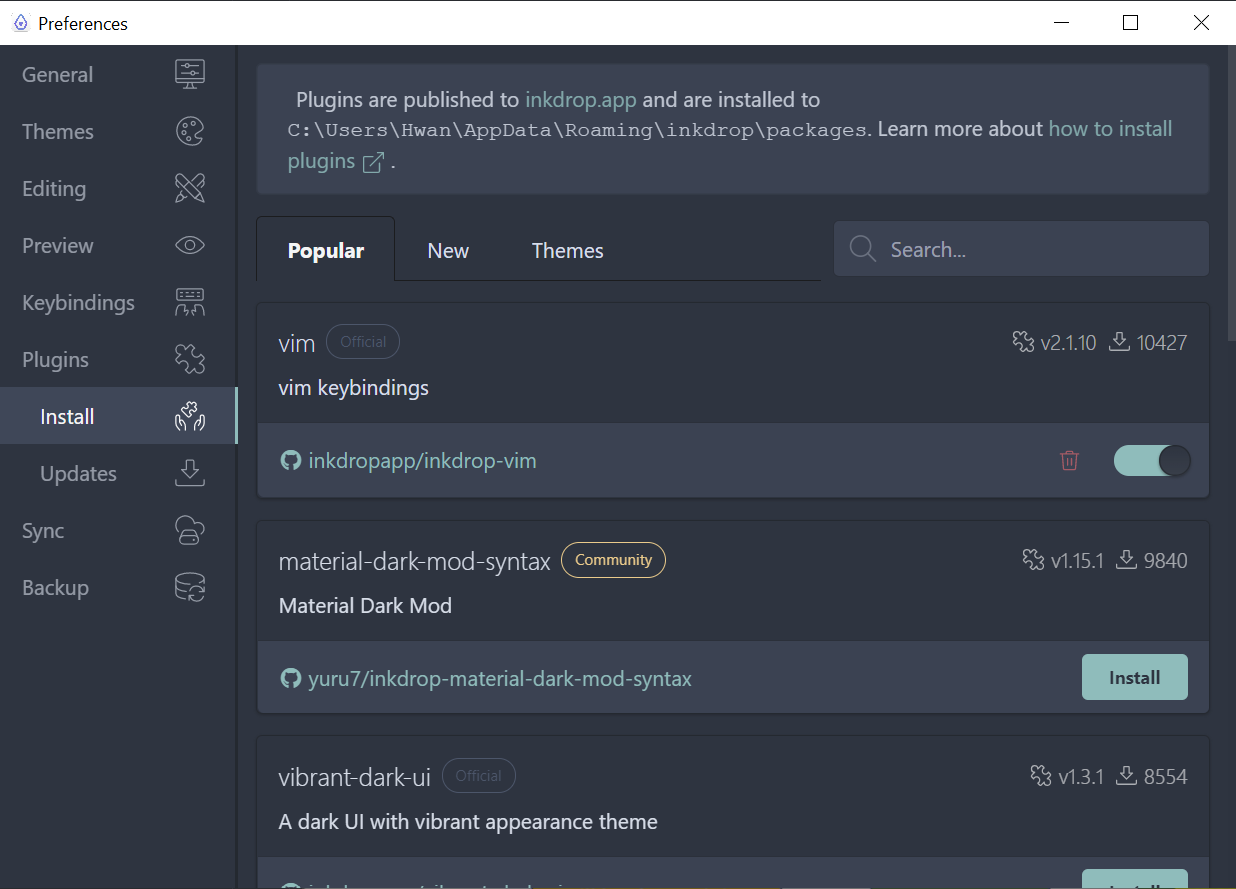
\includegraphics[scale=\figscale]{Figures/inkdrop_vim_plugin.png}
    \caption{Inkdrop Vim plugin}
    \label{FigInkdropVimPlugin}
\end{figure}
To modify the key bindings, following the Inkdrop user manual
\cite{matsuyamacustomizing} you can modify the \textbf{keymap.cson} file which
can be instantly directed to using the following link:
\begin{figure}[H]
    \centering
    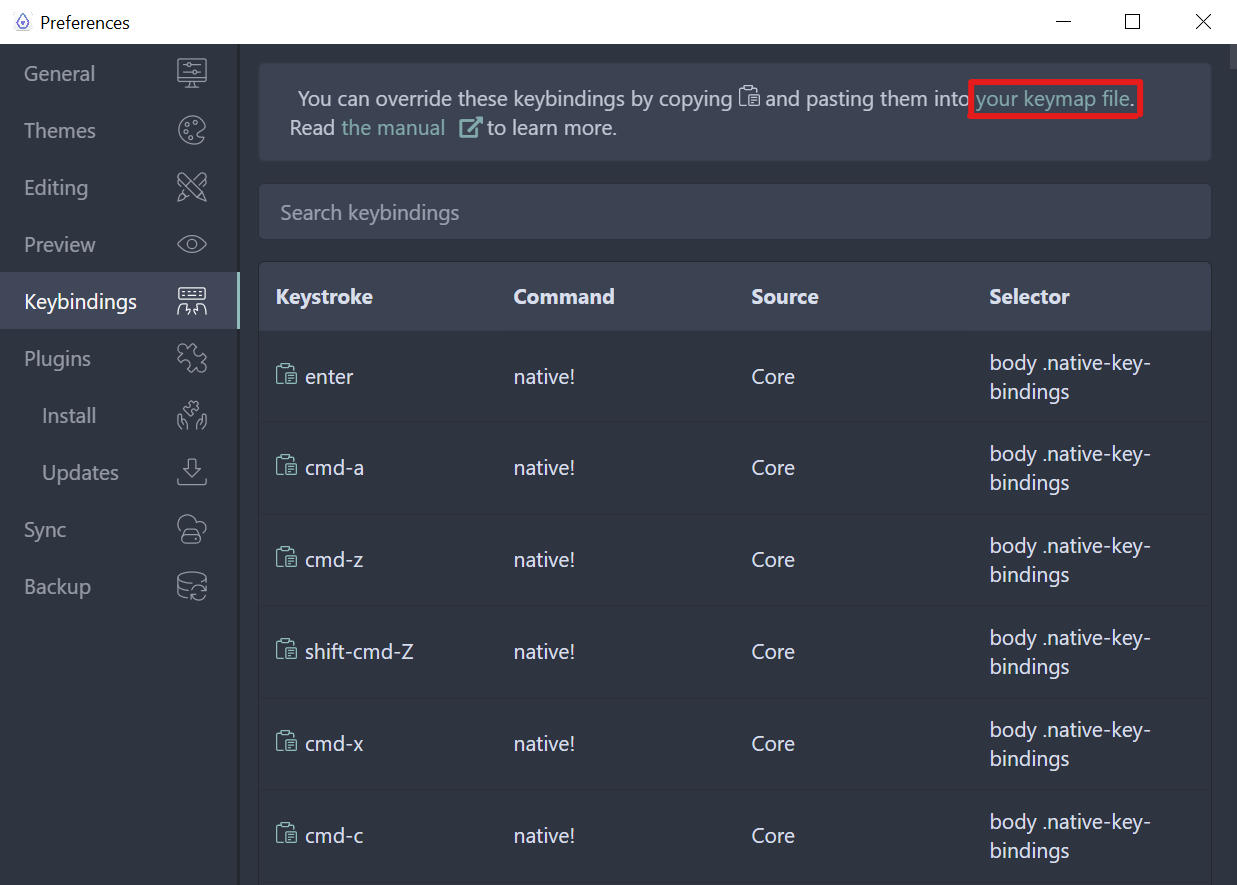
\includegraphics[scale=\figscale]{Figures/inkdrop_keymap_file.png}
    \caption{Inkdrop keymap file link}
    \label{FigInkdropKeymapFile}
\end{figure}
Here is an example of the \textbf{keymap.cson} file:
\begin{lstlisting}
'.CodeMirror.vim-mode:not(.insert-mode):not(.key-buffering) textarea':
  'shift-j': 'vim:scroll-down'
  'shift-k': 'vim:scroll-up'
  'ctrl-j': 'vim:join'
\end{lstlisting}
You can modify this in Vim after navigating to it in terminal and with Inkdrop
on. Any saved changes will be instantly reflected in the app and errors will
result in a popup.\\

To enable relative line numbers, we need to instead modify the \textbf{init.js}
file which can be opened from the settings menu:
\begin{figure}[H]
    \centering
    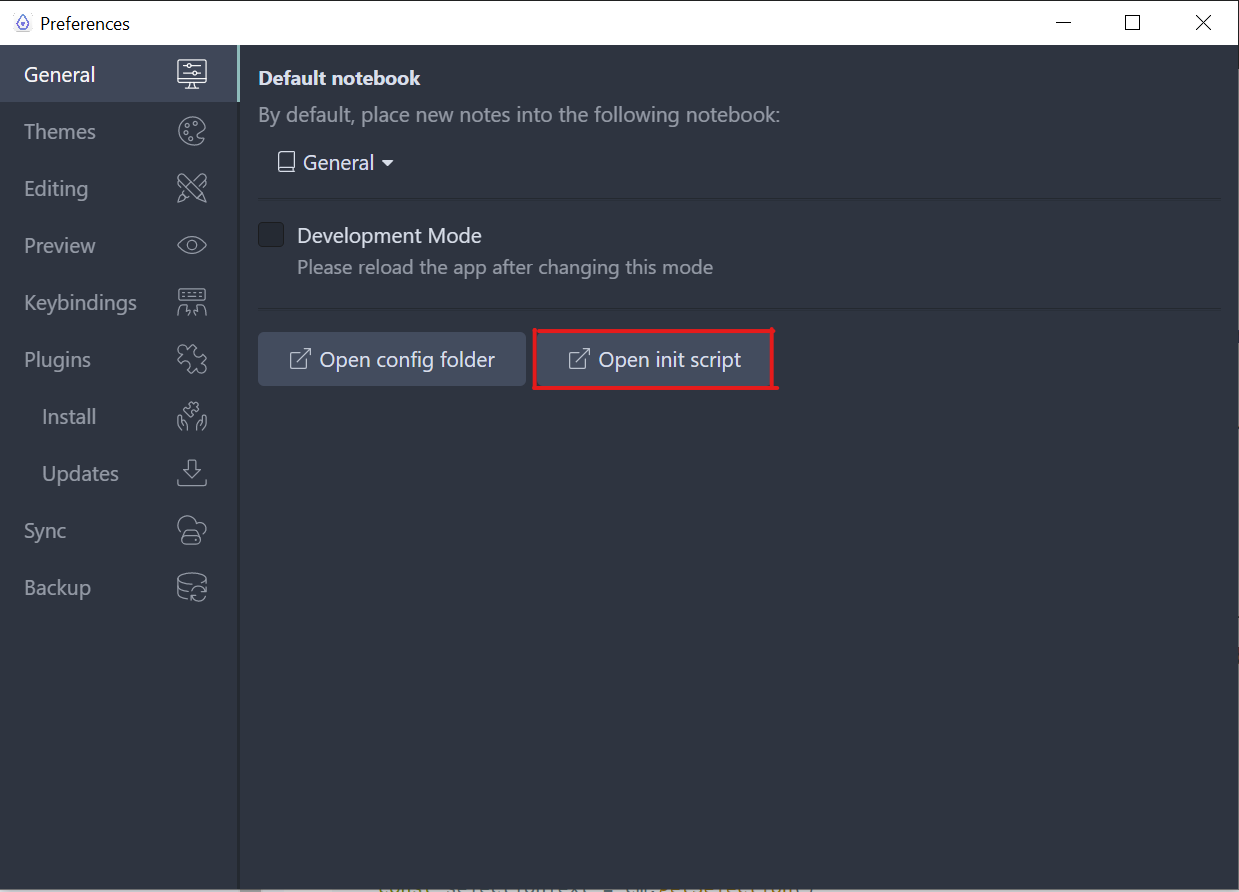
\includegraphics[scale=\figscale]{Figures/inkdrop_init_file.png}
    \caption{Inkdrop init.js file}
    \label{FigInkdropInitFile}
\end{figure}
and add the following:
\begin{lstlisting}
inkdrop.onEditorLoad((editor) => {
  const { cm } = editor

  function showRelativeLines(cm) {
    const lineNum = cm.getCursor().line + 1;
    if (cm.state.curLineNum === lineNum) {
      return;
    }
    cm.state.curLineNum = lineNum;
    cm.setOption('lineNumberFormatter', l =>
      l === lineNum ? lineNum : Math.abs(lineNum - l));
  }
  cm.on('cursorActivity', showRelativeLines)
})
\end{lstlisting}

%==============================================================================
\section{ShareX}
%==============================================================================
The default windows snipping tool is pretty trash. It doesn't even have the
functionality to draw a simple rectangle on a screenshot! Instead, I recommend
ShareX which can be obtained from \cite{sharex}. Other than the ability to
screenshot, it also has the capability to record a section of screen! This is
definitely of my favourite pieces of software!\\

Customization can be done using the UI. You can also import settings if you
wish. To do so, on the left blade, navigate to `Application settings' then
`Settings' as displayed below:
\begin{figure}[H]
    \centering
    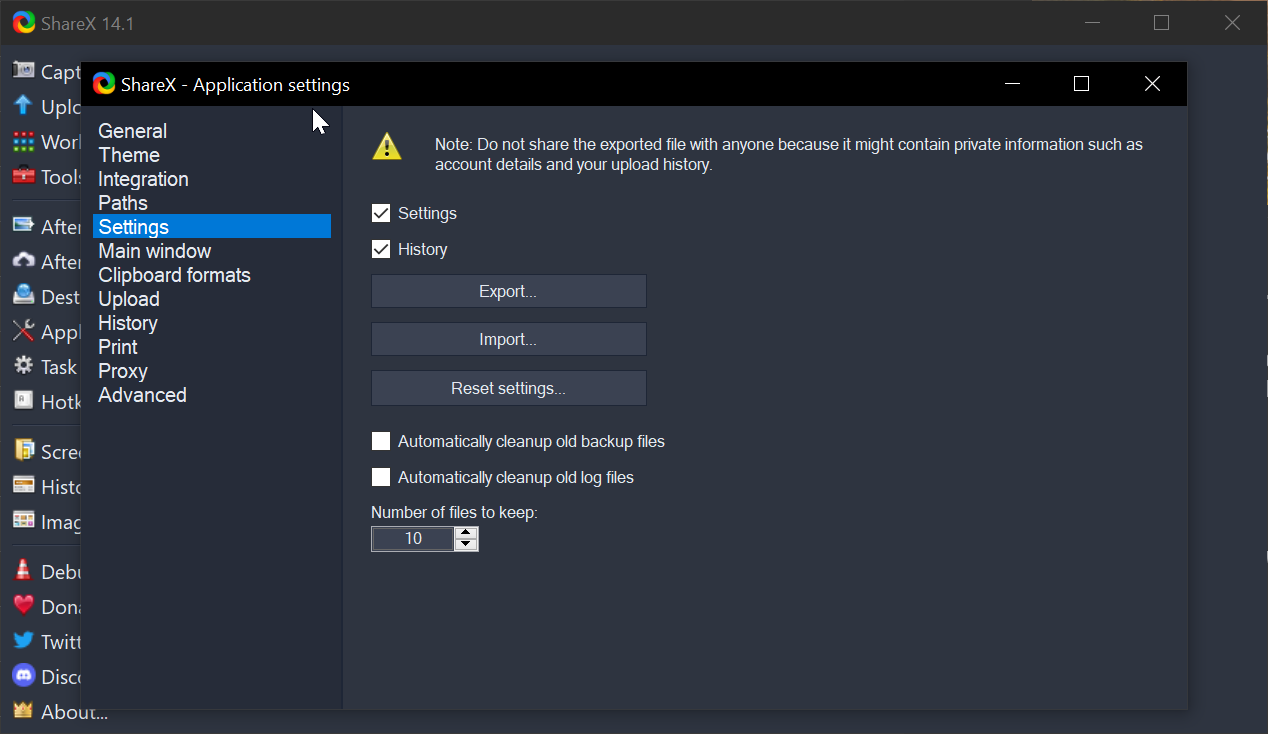
\includegraphics[scale=\figscale]{sharex_settings.png}
    \caption{ShareX settings}
    \label{FigShareXSetting}
\end{figure}

%==============================================================================
\section{Autohotkey Script for Drawing on Screen}
%==============================================================================
Whilst EpicPen is fairly popular, I find that it clashes with my windows
hotkeys. It's also fairly bloated and has advertisements which is unacceptable
to me. Instead, there exist Autohotkey scripts that implement a simple drawing
tool. I found it in the first comment by `Hellbent' in the Autohotkey forum post
\cite{hellbent2019draw}. The keys are simple:
\begin{itemize}
    \item Hold Ctrl and left-click to draw
    \item Use Ctrl and right-click to erase
    \item Use Ctrl and mouse wheel to select colour
\end{itemize}
